\documentclass[english,floatsintext,man]{apa6}

\usepackage{amssymb,amsmath}
\usepackage{ifxetex,ifluatex}
\usepackage{fixltx2e} % provides \textsubscript
\ifnum 0\ifxetex 1\fi\ifluatex 1\fi=0 % if pdftex
  \usepackage[T1]{fontenc}
  \usepackage[utf8]{inputenc}
\else % if luatex or xelatex
  \ifxetex
    \usepackage{mathspec}
    \usepackage{xltxtra,xunicode}
  \else
    \usepackage{fontspec}
  \fi
  \defaultfontfeatures{Mapping=tex-text,Scale=MatchLowercase}
  \newcommand{\euro}{€}
\fi
% use upquote if available, for straight quotes in verbatim environments
\IfFileExists{upquote.sty}{\usepackage{upquote}}{}
% use microtype if available
\IfFileExists{microtype.sty}{\usepackage{microtype}}{}

% Table formatting
\usepackage{longtable,booktabs}
\usepackage[counterclockwise]{rotating}   % Landscape page setup for large tables
\usepackage{multirow}		% Table styling
\usepackage{tabularx}		% Control Column width
\usepackage[flushleft]{threeparttable}	% Allows for three part tables with a specified notes section
\usepackage{threeparttablex}            % Lets threeparttable work with longtable
\usepackage{longtable}              % Allows tables to break across pages

  \usepackage{graphicx}
  \makeatletter
  \def\maxwidth{\ifdim\Gin@nat@width>\linewidth\linewidth\else\Gin@nat@width\fi}
  \def\maxheight{\ifdim\Gin@nat@height>\textheight\textheight\else\Gin@nat@height\fi}
  \makeatother
  % Scale images if necessary, so that they will not overflow the page
  % margins by default, and it is still possible to overwrite the defaults
  % using explicit options in \includegraphics[width, height, ...]{}
  \setkeys{Gin}{width=\maxwidth,height=\maxheight,keepaspectratio}
\ifxetex
  \usepackage[setpagesize=false, % page size defined by xetex
              unicode=false, % unicode breaks when used with xetex
              xetex]{hyperref}
\else
  \usepackage[unicode=true]{hyperref}
\fi
\hypersetup{breaklinks=true,
            pdfauthor={},
            pdftitle={A Quantitative Synthesis of Early Language Acquisition Using Meta-Analysis},
            colorlinks=true,
            citecolor=blue,
            urlcolor=blue,
            linkcolor=black,
            pdfborder={0 0 0}}
\urlstyle{same}  % don't use monospace font for urls

\setlength{\parindent}{0pt}
%\setlength{\parskip}{0pt plus 0pt minus 0pt}

\setlength{\emergencystretch}{3em}  % prevent overfull lines

\setcounter{secnumdepth}{0}
\ifxetex
  \usepackage{polyglossia}
  \setmainlanguage{}
\else
  \usepackage[english]{babel}
\fi

% Manuscript styling
\captionsetup{font=singlespacing,justification=justified}
\usepackage{csquotes}



\usepackage{tikz} % Variable definition to generate author note

% fix for \tightlist problem in pandoc 1.14
\providecommand{\tightlist}{%
  \setlength{\itemsep}{0pt}\setlength{\parskip}{0pt}}

% Essential manuscript parts
  \title{A Quantitative Synthesis of Early Language Acquisition Using
Meta-Analysis}

  \shorttitle{A Quantitative Synthesis}


  \author{
          Molly Lewis\textsuperscript{1},
          Mika Braginsky\textsuperscript{1},
          Sho Tsuji\textsuperscript{2},
          Christina Bergmann\textsuperscript{2},
          Page Piccinini\textsuperscript{2},
          Alejandrina Cristia\textsuperscript{2},
          Michael C. Frank\textsuperscript{1}  }

  \def\affdep{{"", "", "", "", "", "", ""}}%
  \def\affcity{{"", "", "", "", "", "", ""}}%

  \affiliation{
    \vspace{0.5cm}
          \textsuperscript{1} Department of Psychology, Stanford University\\
          \textsuperscript{2} Laboratoire de Sciences Cognitives et Psycholinguistique, ENS  }


%   \def\affinst{{"init", "Department of Psychology, Stanford University", "Laboratoire de Sciences Cognitives et Psycholinguistique, ENS"}}%
%   \def\affstate{{"init", "", ""}}%
%   \def\affcntry{{"init", "", ""}}%

  \note{
    \vspace{1cm}
    Author note

    \raggedright
    \setlength{\parindent}{0.4in}

    \newcounter{author}

%     %     %       %       \setcounter{author}{0}
%         %           \addtocounter{author}{1}
%         %         \expandafter\edef\csname authorid\endcsname{\theauthor}
%         Molly Lewis, \pgfmathparse{\affdep[\authorid]} \pgfmathresult, \pgfmathparse{\affinst[\authorid]} \pgfmathresult, \pgfmathparse{\affcity[\authorid]} \pgfmathresult, \pgfmathparse{\affstate[\authorid]} \pgfmathresult, \pgfmathparse{\affcntry[\authorid]} \pgfmathresult
%       %     ;
%     %       %       \setcounter{author}{0}
%         %           \addtocounter{author}{1}
%         %         \expandafter\edef\csname authorid\endcsname{\theauthor}
%         Mika Braginsky, \pgfmathparse{\affdep[\authorid]} \pgfmathresult, \pgfmathparse{\affinst[\authorid]} \pgfmathresult, \pgfmathparse{\affcity[\authorid]} \pgfmathresult, \pgfmathparse{\affstate[\authorid]} \pgfmathresult, \pgfmathparse{\affcntry[\authorid]} \pgfmathresult
%       %     ;
%     %       %       \setcounter{author}{0}
%         %           \addtocounter{author}{2}
%         %         \expandafter\edef\csname authorid\endcsname{\theauthor}
%         Sho Tsuji, \pgfmathparse{\affdep[\authorid]} \pgfmathresult, \pgfmathparse{\affinst[\authorid]} \pgfmathresult, \pgfmathparse{\affcity[\authorid]} \pgfmathresult, \pgfmathparse{\affstate[\authorid]} \pgfmathresult, \pgfmathparse{\affcntry[\authorid]} \pgfmathresult
%       %     ;
%     %       %       \setcounter{author}{0}
%         %           \addtocounter{author}{2}
%         %         \expandafter\edef\csname authorid\endcsname{\theauthor}
%         Christina Bergmann, \pgfmathparse{\affdep[\authorid]} \pgfmathresult, \pgfmathparse{\affinst[\authorid]} \pgfmathresult, \pgfmathparse{\affcity[\authorid]} \pgfmathresult, \pgfmathparse{\affstate[\authorid]} \pgfmathresult, \pgfmathparse{\affcntry[\authorid]} \pgfmathresult
%       %     ;
%     %       %       \setcounter{author}{0}
%         %           \addtocounter{author}{2}
%         %         \expandafter\edef\csname authorid\endcsname{\theauthor}
%         Page Piccinini, \pgfmathparse{\affdep[\authorid]} \pgfmathresult, \pgfmathparse{\affinst[\authorid]} \pgfmathresult, \pgfmathparse{\affcity[\authorid]} \pgfmathresult, \pgfmathparse{\affstate[\authorid]} \pgfmathresult, \pgfmathparse{\affcntry[\authorid]} \pgfmathresult
%       %     ;
%     %       %       \setcounter{author}{0}
%         %           \addtocounter{author}{2}
%         %         \expandafter\edef\csname authorid\endcsname{\theauthor}
%         Alejandrina Cristia, \pgfmathparse{\affdep[\authorid]} \pgfmathresult, \pgfmathparse{\affinst[\authorid]} \pgfmathresult, \pgfmathparse{\affcity[\authorid]} \pgfmathresult, \pgfmathparse{\affstate[\authorid]} \pgfmathresult, \pgfmathparse{\affcntry[\authorid]} \pgfmathresult
%       %     ;
%     %       %       \setcounter{author}{0}
%         %           \addtocounter{author}{1}
%         %         \expandafter\edef\csname authorid\endcsname{\theauthor}
%         Michael C. Frank, \pgfmathparse{\affdep[\authorid]} \pgfmathresult, \pgfmathparse{\affinst[\authorid]} \pgfmathresult, \pgfmathparse{\affcity[\authorid]} \pgfmathresult, \pgfmathparse{\affstate[\authorid]} \pgfmathresult, \pgfmathparse{\affcntry[\authorid]} \pgfmathresult
%       %     .
%     
    Correspondence concerning this article should be addressed to Molly
    Lewis, Psychology Department, Stanford University. 450 Serra Mall,
    Stanford, CA 94305. E-mail:
    \href{mailto:mll@stanford.edu}{\nolinkurl{mll@stanford.edu}}.

                                                                                    }

  \keywords{developmental psychology, language acquisition, quantitative theories,
meta-analysis \\

    \indent Word count: XXXX
  }

  \usepackage{setspace}
  \usepackage{float}
  \usepackage{graphicx}
  \AtBeginEnvironment{tabular}{\singlespacing}
  \usepackage{pbox}

\begin{document}

\maketitle



\section{Introduction}\label{introduction}

To learn to speak a language, a child must acquire a wide range of
knowledge and skills: the sounds of the language, the word forms, and
the mappings of words to meanings, to name only a few. How does this
process unfold? Our goal as psychologists is to build a broad theory
that can explain and predict this process. An important aspect of this
theory is an account of how the acquisition of individual skills depends
on other skills. For example, the theory must describe to what extent a
child must master language sounds before beginning the process of
learning the meanings of words. To develop this theory, a pragmatic
research strategy has been to study skills primarily in isolation,
describing the developmental trajectories of individual phenomena in
separate research programs. This research shows that, while the onset of
these skills can often be found in the first year of life, most follow a
protracted pattern of development, with important changes occurring in
the second year and beyond. Importantly, however, if linguistic skills
are in fact interdependent, then there is reason to question results
based on the isolationist method, and suggests that we will not be able
to understand individuals skills without a more precise understanding of
the broader system.

The theory building effort is further complicated by the fact that we
typically have some uncertainty about the trajectory of individual
skills. Developmental trajectories are often communicated as verbal
descriptions that summarize a body of noisy experimental findings.
However, in actual fact, there is often one study finding an effect, but
another failing to do so. These contradictions leave the theorist with
uncertainty about which experimental findings should constrain the
theory, which is often resolved by verbally discounting one or the other
finding depending on the viewer's expertise (and potentially theoretical
penchant). What is needed then is a method for resolving these
contradictions in a more systematic and principled fashion.

We suggest a solution to both of these challenges---building integrative
whole-system views and evaluating evidential strength in a field of
scientific research---is to describe experimental findings in
quantitative, rather than qualitative, terms. Quantitative descriptions
allow for the use of quantitative methods for aggregating experimental
findings in order to evaluate evidential strength. In addition,
describing experimental findings as quantitative estimates provides a
common language for comparing across phenomena, and a way to make more
precise predictions. In this paper, we consider the domain of language
acquisition and demonstrate how the quantitative tools of meta-analysis
can support theory building in psychological research.

Meta-analysis is a quantitative method for aggregating across
experimental findings. The fundamental unit of meta-analysis is the
\emph{effect size}: a scale-free, quantitative measure of
\enquote{success} in a phenomenon. Importantly, an effect size provides
an estimate of the \emph{size} of an effect, as well as a measure of
uncertainty around this point estimate. With such a quantitative measure
of success, we can apply the same reasoning we use to aggregate noisy
measurements over participants in a single study: By assuming each
\emph{study}, rather than participant, is sampled from a population, we
can appeal to a statistical framework to combine estimates of the effect
size for a given phenomenon.

Meta-analytic methods support theory building in several ways. First,
they provide a way to evaluate which effects in a literature are most
likely to be observed consistently, and thus should constrain the
theory. This issue is particularly important in light of recent
high-profile evidence that an effect observed in one study may not
replicate in another (``replication crisis,'' Ioannidis, 2005; Open
Science Collaboration, 2012, 2015). Failed replications are difficult to
interpret, however, because they may result from a wide variety of
causes, including an initial false positive, a subsequent false
negative, or differences between initial and replication studies, such
that making causal attributions in a situation with two conflicting
studies is often difficult (Anderson et al., 2016; Gilbert, King,
Pettigrew, \& Wilson, 2016). By aggregating evidence across studies and
assuming that there is some variability in true effect size from study
to study, meta-analytic methods can provide a more veridical description
of the empirical landscape, which in turn leads to better
theory-building.

Second, meta-analysis supports theory building by providing higher
fidelity descriptions of phenomena. Given an effect size estimate,
meta-analytic methods provide a method for quantifying the amount
variability around this point estimate. Furthermore, the quantitative
framework allows researchers to detect potential moderators in effect
size. This ability is particularly important for developmental phenomena
because building a theory requires a precise description of changes in
effect size across development. Individual papers typically describe an
effect size for 1-2 age groups, but the ultimate goal is to detect a
moderator---age---in this effect. Given that moderators always require
more power to detect (Button et al., 2013), it may be quite difficult to
identify developmental trends in effect sizes from individual papers. By
aggregating across papers using meta-analytic methods, however, we may
be able to detect these changes, leading to a more precise description
of the empirical phenomena.

Finally, effect size estimates also provide a common language for
comparing \emph{across} phenomena. In the current work, this common
language allows us to meaningfully consider the relationship between
different phenomena in the language acquisition domain
(\enquote{meta-meta-analysis}). Through cross-phenomena comparisons, we
can understand not only the trajectory of a particular phenomenon, such
as word learning, but also how the trajectory of each phenomenon might
relate to other skills, such as sound learning, gaze following, and many
others. This more holistic description of the empirical landscape can
inform theories about the extent to which there is interdependence
between the acquisition of different linguistic skills.

Meta-analytic tools are broadly applicable to psychological literatures,
but developmental research may be a particularly informative application
of these tools. One reason is that developmental studies may be uniquely
vulnerable to false findings because running children is expensive, and
thus sample sizes are small and studies are underpowered (Ioannidis,
2005). In addition, the high cost and practical difficulties associated
with collecting large developmental datasets means that replications are
relatively rare in the field. Finally, there has been attention to
research practices in developmental psychology, suggesting evidence of
experimenter bias (Peterson, 2016).

We take as our ultimate goal a broad theory of language acquisition that
can explain and predict the range of linguistic skills a child acquires.
Toward this end, we developed a dataset of effect sizes in the language
acquisition literature across 12 phenomena
(\href{http://metalab.stanford.edu}{Metalab;
http://metalab.stanford.edu/}). We demonstrate how meta-analysis
supports building this theory in three ways. We first use meta-analytic
techniques to evaluate the evidential value of the empirical landscape
in language acquisition research. We find broadly that this literature
has strong evidential value, and thus that the effects reported in the
literature should constrain our theorizing of language acquisition. We
then turn toward the task of synthesizing these findings across
phenomena and finally offer an example of quantitative evaluation of
theories.

\section{Method}\label{method}

We analyzed 12 different phenomena in language acquisition. To a certain
extent, these phenomena were selected opportunistically, either because
of high prevalence in the literature or because a published
meta-analysis already existed. The phenomena cover development at many
different levels of the language hierarchy, from the acquisition of
prosody and phonemic contrasts, to gaze following in communicative
interaction. This wide range of phenomena allowed us to compare the
course of development across different domains, as well as to explore
questions about the interactive nature of language acquisition (Table
1).

To obtain estimates of effect size, we either coded or adapted others'
coding of papers reporting experimental data (see SI for details).
Within each paper, we calculated a separate effect size estimate for
each experiment and age group (we refer to this as a
\enquote{condition}). In total, our sample includes estimates from 231
papers, 881 different conditions and 10,741 participants. The process
for selecting papers from the literature differed by domain, with some
individual meta-analyses using more systematic approaches than others
(see SI). \renewcommand{\arraystretch}{1.5}

\begin{table}[h!]
        \footnotesize
        \begin{tabular}{lp{4cm} p{5cm}r}
            \toprule
            \textbf{Level} & \textbf{Phenomenon}                                                               & \textbf{Description}                                                                                 & \textbf{N papers (conditions)}                                                                                                                                               \\
                        \midrule

            Prosody        & IDS  preference  \newline  {\scriptsize (Dunst, Gorman, \& Hamby, 2012)}          & {\scriptsize  Looking times as a function of whether infant-directed vs. adult-directed speech is presented as stimulation.}      & 16 (50)     \\
            Sounds         & Phonotactic learning  \newline {\scriptsize (Cristia, in prep.)}                   & {\scriptsize Infants' ability to learn phonotactic generalizations from a short exposure.  }                  & 15 (47)                               \\
            ~              & Vowel discrimination (native) \newline {\scriptsize (Tsuji \& Cristia, 2014)}     & {\scriptsize Discrimination of native-language vowels, including results from a variety of methods.  }         & 32 (143)             \\ 
            ~              & Vowel discrimination (non-native) \newline {\scriptsize (Tsuji \& Cristia, 2014)} & {\scriptsize Discrimination of non-native vowels, including results from a variety of methods.  }     & 15 (48)     \\
               & Statistical sound learning  \newline {\scriptsize (Cristia, in prep.)}             & {\scriptsize Infants' ability to learn sound categories from their acoustic distribution.   }  & 11 (40) \\ 
            & Word segmentation \newline {\scriptsize  (Bergmann \& Cristia, 2015) }            & {\scriptsize Recognition of familiarized words from running, natural speech using behavioral methods.  }                     & 66 (291)                                     \\
            Words     &   Mutual exclusivity \newline {\scriptsize (Lewis \& Frank, in prep.)} &{\scriptsize  Bias to assume that a novel word refers to a novel object.}
            & 20 (60)             \\
            ~ &   Sound Symbolism \newline {\scriptsize (Lammertink et al., 2016)} &{\scriptsize  Bias to assume a non-arbitrary relationship between form and meaning ("bouba-kiki effect").}
            & 10 (42)             \\
            ~              & Concept-label advantage   \newline {\scriptsize (Lewis \& Long, unpublished)}     & {\scriptsize Infants' categorization judgments in the presence and absence of labels.    } & 16 (100) \\
            ~              & Online word recognition \newline {\scriptsize (Frank, Lewis, \& MacDonald, 2016)} & {\scriptsize Online word recognition of familiar words using two-alternative forced choice preferential looking.   }              & 6 (15)                         \\
            Communication  & Gaze following  \newline {\scriptsize  (Frank, Lewis, \& MacDonald, 2016)}        & {\scriptsize Gaze following using standard multi-alternative forced-choice paradigms.   }                       & 12 (33)                                           \\
            ~              & Pointing and vocabulary  \newline {\scriptsize (Colonnesi et al., 2010)}          & {\scriptsize Concurrent correlations between pointing and vocabulary..}  & 12 (12)                         \\ 
            \bottomrule
        \end{tabular}
        \caption{Overview of meta-analyses in dataset.}
    \end{table}

\section{Replicability of the field}\label{replicability-of-the-field}

To assess the replicability of language acquisition phenomena, we
conducted several diagnostic analyses: Meta-analytic estimates of effect
size, fail-safe-N (Orwin, 1983), funnel plots, and p-curve (Simonsohn,
Nelson, \& Simmons, 2014b, 2014a; Simonsohn, Simmons, \& Nelson, 2015).
These analytical approaches each have limitations, but taken together,
they provide converging evidence about whether a true effect is likely
to exist, and the extent to which publication bias and other
questionable research practices are present in the literature. Overall,
we find most phenomena in the language acquisition literature have
evidential value, and should therefore provide the basis for theoretical
development. We also find evidence for some bias, as well as evidence
that two phenomena---phonotactic learning and statistical sound
learning---likely describe null or near-null effects.

\subsection{Meta-Analytic Effect Size}\label{meta-analytic-effect-size}

To estimate the overall effect size of a literature, effect sizes are
pooled across papers to obtain a single meta-analytic estimate. This
meta-analytic effect-size can be thought of as the \enquote{best
estimate} of the effect size for a phenomenon given all the available
data in the literature.

Table 2, column 2 presents meta-analytic effect size estimates for each
of our phenomena. We find evidence for a non-zero effect size in 11 out
of 12 of the phenomena in our dataset, suggesting these literatures
provide evidential value. In the case of phonotactic learning, however,
we find that the meta-analytic effect size estimate does not differ from
zero, suggesting that this literature does not describe a robust effect.

We next turn to methods of assessing evidential value that describe the
\emph{degree} to which a literature has evidential value, and thus the
degree to which it should constrain our theory building. In the
following three analyses---fail-safe-N, funnel plots, and p-curves---we
attempt to quantify the evidential value of these literatures.

\subsection{Fail-safe-N}\label{fail-safe-n}

One approach for quantifying the reliability literature is to ask, How
many missing studies with null effects would have to exist in the
\enquote{file drawer} in order for the overall effect size to be zero?
This is called the \enquote{fail-safe} number of studies (Orwin, 1983).
This number provides an estimate of the size and variance of an effect
using the intuitive unit of studies. To estimate this number, we
estimated the overall effect size for each phenomenon (Table 2, column
2), and then used this to estimate the fail-safe-N (Table 2, column 3).

Because of the large number of positive studies in many of the
meta-analyses we assessed, this analysis suggests a very large number of
studies would have to be \enquote{missing} in each literature (\(M\) =
3622) in order for the overall effect sizes to be 0. Thus, while it is
possible that some reporting bias is present in the literature, the
large fail-safe-N suggests that the literature nonetheless likely
describes a real effect.

This analysis provides a quantitative estimate of the size of an effect
in an intuitive unit, but it does not assess analytical or publication
bias (CITE). Importantly, if experimenters are exercising analytical
flexibility through practices like selective reporting and p-hacking,
then the number and magnitude of observed true effects in the literature
may be greatly inflated. In the next analysis, we assess the presence of
bias through funnel plots.

\subsection{Funnel Plots}\label{funnel-plots}

Funnel plots provide a visual method for evaluating whether variability
in effect sizes is due only to differences in sample size. A funnel plot
shows effect sizes versus a metric of sample size, standard error. If
there is no bias in a literature, we should expect studies to be
randomly sampled around the mean, with more variability for less precise
studies.

Figure 1 presents funnel plots for each of our 12 meta-analyses. These
plots show evidence of asymmetry (bias) for several of our phenomenon
(Table 2, column 4). However, an important limitation of this method is
that it is difficult to determine the source of this bias. One
possibility is that this bias reflects true heterogeneity in phenomena
(e.g.~different
ages)\footnote{The role of moderators such as age can be interactively explored on the MetaLab website (www.metalab.stanford.edu).}.
P-curve analyses provide one method for addressing this issue, which we
turn to next.

\begin{figure}[htbp]
\centering
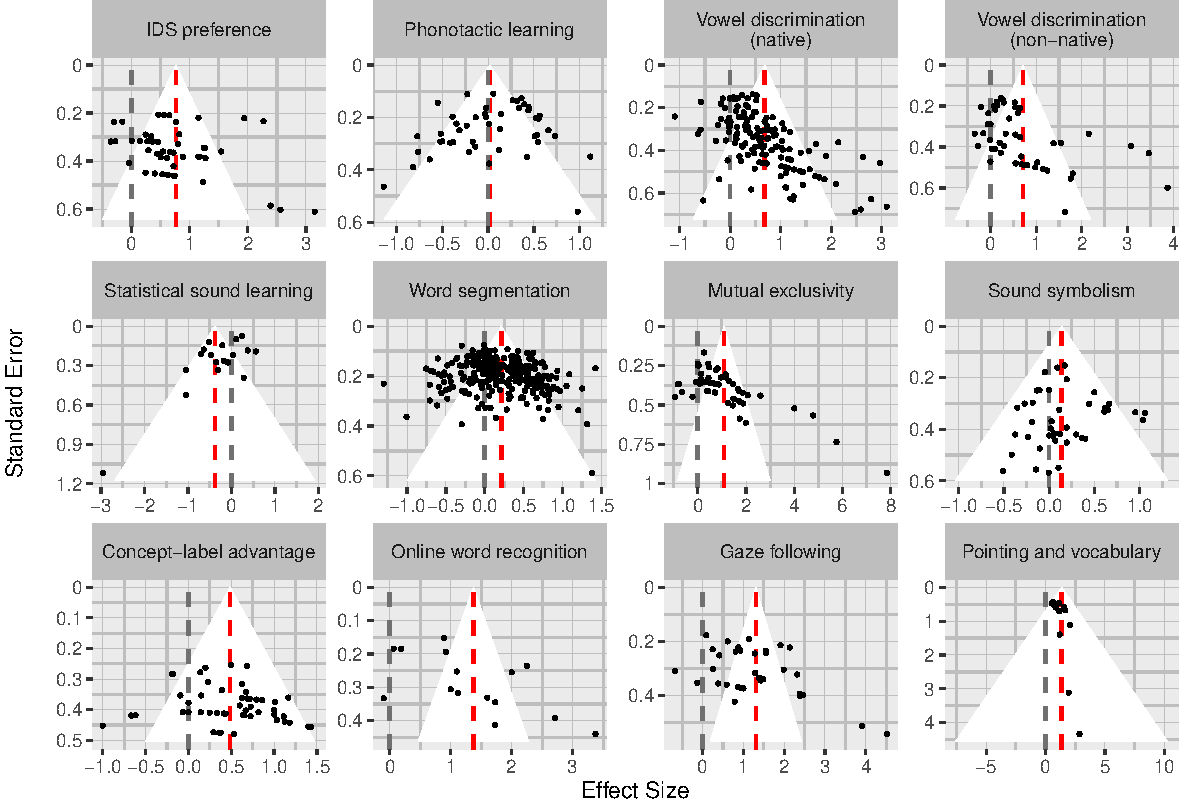
\includegraphics{metalab_synthesis_files/figure-latex/unnamed-chunk-2-1.pdf}
\caption{Funnel plots for each meta-analysis. Each effect size estimate
is represented by a point, and the mean effect size is shown as a red
dashed line. The grey dashed line shows an effect size of zero. The
funnel corresponds to a 95\% CI around this mean. In the absence of true
heterogeneity in effect sizes (no moderators) and bias, we should expect
all points to fall inside the funnel.}
\end{figure}

\subsection{P-curves}\label{p-curves}

\begin{figure}[htbp]
\centering
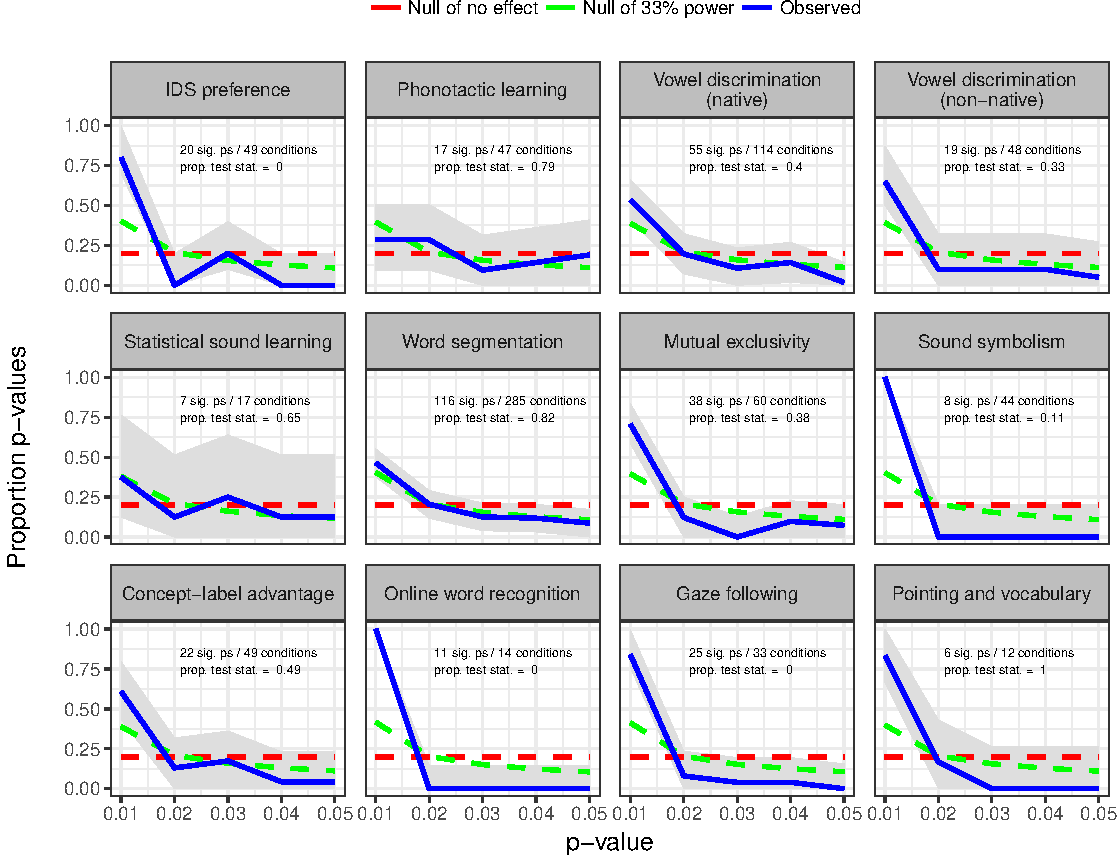
\includegraphics{metalab_synthesis_files/figure-latex/p_curve_plots-1.pdf}
\caption{P-curve for each meta-analysis (Simonsohn, Nelson, \& Simmons,
2014), except those for which p-values were unavailable. In the absense
of p-hacking, we should expect the observed p-curve (blue) to be
right-skewed (more small values). The red dashed line shows the expected
distribution of p-values when the effect is non-existent (the null is
true). The green dashed line shows the expected distribution if the
effect is real, but studies only have 33\% power.}
\end{figure}

A p-curve is the distribution of p-values for the statistical test of
the main hypothesis across a literature (Simonsohn et al., 2014b, 2014a,
2015). Critically, if there is a robust effect in the literature, the
shape of the p-curve should reflect this. In particular, we should
expect the p-curve to be right-skewed with more small values (e.g., .01)
than large values (e.g., .04). An important property of this analysis is
that we should expect this skew independent of any true heterogeneity in
the data, such as age. Evidence that the curve is in fact right-skewed
would suggest that the literature is not biased, and that it provides
evidential value for theory building.

\begin{table}[t]
\footnotesize
\begin{tabular}{lrrrr}
\toprule
\textbf{Phenomenon} & \textbf{\textit{d}} & \textbf{fail-safe-N} & \textbf{funnel skew} & \textbf{p-curve skew}\\
\midrule

IDS preference & 0.72 [0.54, 0.91] & 3762 & 1.26 (0.21) & 1.26 (0.21)\\
Phonotactic learning & 0.04 [-0.09, 0.16] & 45 & -1.08 (0.28) & -1.08 (0.28)\\
Vowel discrimination (native) & 0.59 [0.49, 0.7] & 9620 & 8.87 (< .01) & 8.87 (< .01)\\
Vowel discrimination (non-native) & 0.66 [0.42, 0.9] & 3391 & 4.13 (< .01) & 4.13 (< .01)\\
Statistical sound learning & -0.13 [-0.25, -0.01] & na & -1.58 (0.11) & -1.58 (0.11)\\
Word segmentation & 0.2 [0.16, 0.25] & 5930 & 2.61 (0.01) & 2.61 (0.01)\\
Mutual exclusivity & 1.01 [0.68, 1.33] & 6443 & 6.25 (< .01) & 6.25 (< .01)\\
Sound symbolism & 0.15 [0.04, 0.26] & 538 & -1.32 (0.19) & -1.32 (0.19)\\
Concept-label advantage & 0.4 [0.29, 0.51] & 3928 & 0.31 (0.76) & 0.31 (0.76)\\
Online word recognition & 1.34 [0.86, 1.82] & 2043 & 2.16 (0.03) & 2.16 (0.03)\\
Gaze following & 0.81 [0.24, 1.38] & 2527 & -1.66 (0.1) & -1.66 (0.1)\\
Pointing and vocabulary & 0.98 [0.62, 1.34] & 1617 & 1.15 (0.25) & 1.15 (0.25)\\


\bottomrule
\end{tabular}
\caption{Summary of replicability analyses. \textit{d} = Effect size (Cohen's {\it d}) estimated from a random-effect model; fail-safe-N = number of missing studies that would have to exist in order for the overall effect size to be {\it d} = 0; funnel skew = test of asymmetry in funnel plot using the random-effect Egger's test (Stern \& Eggers, 2005); p-curve skew = test of the right skew of the p-curve using the Stouffer method (Simonsohn, Simmons, \& Nelson, 2015); Brackets give 95\% confidence intervals, and parentheses show p-values.}
\end{table}

Figure 2 shows p-curves for 12 of our 12
meta-analyses.\footnote{We did not conduct p-curves on all meta-analyses because previously published meta-analyses did not include the original test statistics in the summary report (IDS preference and pointing and vocabulary). In other cases, the key test statistics were inappropriate for p-curve (online word recognition and gaze following).}
With the exception of phonotactic learning, all p-curves show evidence
of right skew (Table 2, column 5).

In sum, then, meta-analytic methods, along with our dataset of effect
sizes, provide an opportunity to assess the replicability of the field
of language acquisition. Across a range of analyses, we find that this
literature shows some evidence for bias, but overall, it is quite
robust.

\section{Quantitative Evaluation of
Theories}\label{quantitative-evaluation-of-theories}

Next, we turn to how these data can be used to constrain and develop
theories of language acquisition.

Meta-analytic methods provide a precise, quantitative description of the
developmental trajectory of individual phenomena. Figure 3 presents the
developmental trajectories of the phenomena in our dataset at each level
in the linguistic
hierarchy.\footnote{The pointing and vocabulary dataset is excluded from this analysis because it does not contain effect sizes at multiple ages.}
By describing how effect sizes change as a function of age, we can begin
to understand what factors might moderate that trajectory, such as
aspects of a child's experience or maturation. For example, the
meta-analysis on mutual-exclusivity (the bias for children to select a
novel object, given a novel word; Markman \& Wachtel, 1988) suggests a
steep developmental trajectory of this skill. We then can use these data
to build quantitative models to understand how aspects of experience
(e.g.~vocabulary development) or maturational constraints may be related
to this trajectory (e.g., Frank, Goodman, \& Tenenbaum, 2009; McMurray,
Horst, \& Samuelson, 2012).

\begin{figure}[htbp]
\centering
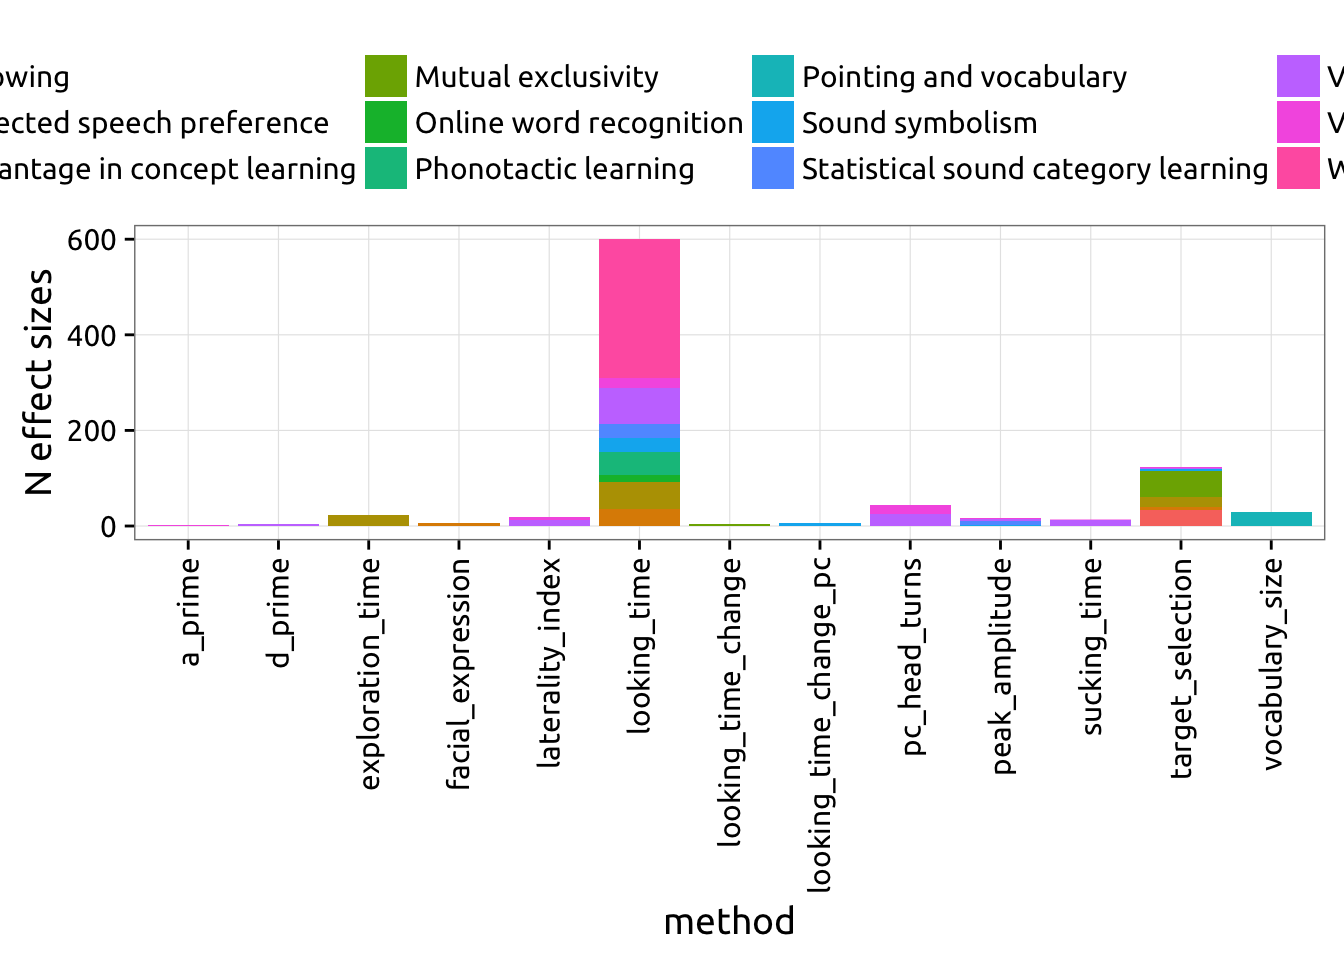
\includegraphics{metalab_synthesis_files/figure-latex/unnamed-chunk-3-1.pdf}
\caption{Method-residual effect size plotted as a function of age across
all developmental meta-analyses in our dataset. Lines show logarithmic
model fits. Each point corresponds to a condition, with the size of the
point indicating the number of participants. {[}fix labels manually;
deal with communication{]}}
\end{figure}

\begin{figure}[htbp]
\centering
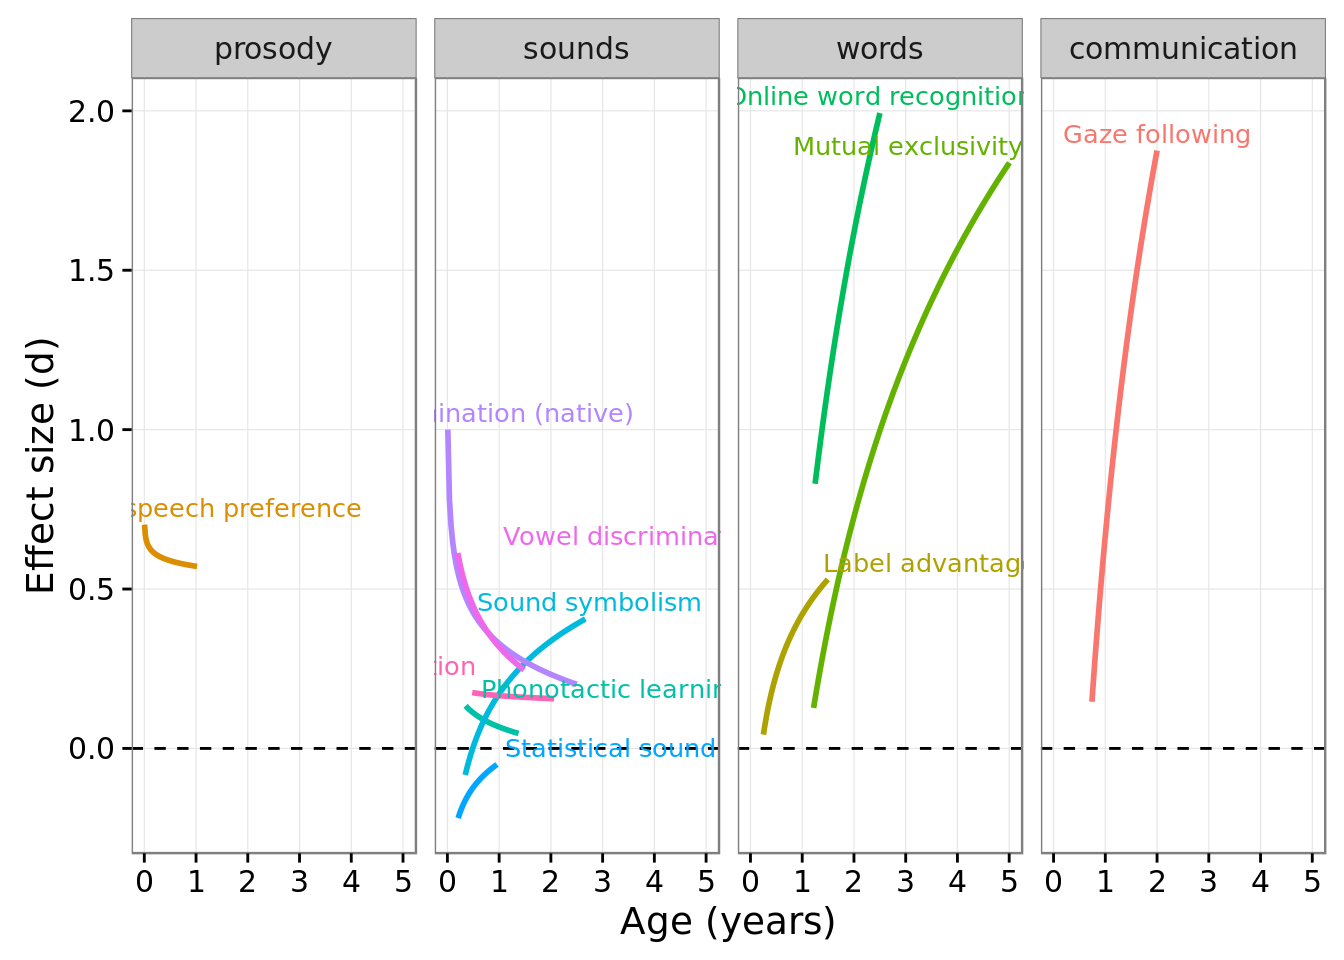
\includegraphics{metalab_synthesis_files/figure-latex/unnamed-chunk-4-1.pdf}
\caption{The left two panels show the developmental trajectories
predicted under different meta-theories of language acqusition. The
stage-like theory predicts that a child will not begin learning the next
skill in the linguistic hierarchy until the previous skill has been
mastered. The interactive theory predicts that multiple skills may be
simultaneously acquired. The third panel shows other possible
developmental trajectories for an particular phenomenon (decreasing,
linear, and non-monotonic). The fourth panel shows the observed
meta-analytic data. Effect size is plotted as a function of age from 0-3
years, across 12 different phenomena. Model fits are the same as in
Figure 3. These developmental curves suggest there is interactivity
across language skills, rather than stage-like learning of the
linguistic hierarchy.}
\end{figure}

In addition, meta-analytic methods provide an approach for synthesizing
across different linguistic skills via the language of effect sizes. The
ultimate goal is to use meta-analytic data to build a single,
quantitative model of the language acquisition system, much like those
developed for individual language acquisition phenomena, like word
learning. Developing a single quantitative model is a lofty goal,
however, and will likely require much more precise description of the
phenomena than is available in our dataset. Nevertheless, we can use our
data to distinguish between broad meta-theories about the
interdependency of skills.

We first consider two intuitive theories of task-to-task dependencies
that have been articulated in a number of forms. The stage-like theory
proposes that linguistic skills are acquired sequentially beginning with
skills at the lowest level of the linguistic hierarchy. Under this
theory, once a skill is mastered, it can be used to support the
acquisition of skills higher in the linguistic hierarchy. In this way, a
child sequentially acquires the skills of language,
\enquote{bootstrapping} from existing knowledge at lower levels to new
knowledge at higher levels. There is a wide range of evidence consistent
with this view. For example, there is evidence that prosody supports the
acquisition of sound categories {[}CITE{]}, word boundaries {[}CITE{]},
and even word learning (e.g., Shukla, White, \& Aslin, 2011).

A second possibility is that there is interactivity in the language
system such that multiple skills are learned simultaneously across the
system. For example, under this proposal, a child does not wait to begin
learning the meanings of words until the sounds of a language are
mastered; rather, the child is jointly solving the problem of word
learning in concert with other language skills. This possibility is
consistent with predictions of a class of hierarchical Bayesian models
that suggest that more abstract knowledge may be acquired quickly,
before lower level information, and may in turn support the acquisition
of lower information (``blessing of abstraction,'' Goodman, Ullman, \&
Tenenbaum, 2011). There is evidence for this proposal from work that
suggests word learning supports the acquisition of lower-level
information like phonemes (Feldman, Myers, White, Griffiths, \& Morgan,
2013). More broadly, there is evidence that higher level skills like
word learning may be acquired relatively early in development, likely
before lower level skills have been mastered (e.g., Bergelson \&
Swingley, 2012).

These two theories make different predictions about relative
trajectories of skills across development. Within the meta-analytic
framework, we can represent these different trajectories schematically
by plotting the effect sizes for different skills across development. In
particular, the bottom-up theory predicts serial acquisition of skills
(Figure 4; left) while the interactive theory predicts simultaneous
acquisition (left center). We can also specifify many other possible
trajectories by varying the functional form and parameters of the model.
Figure 4 (right center; \enquote{ad hoc}) shows several other possible
trajectories. For example, a skill might have a non-monotonic
trajectory, increasing with age, and then decreasing. By specifying the
shape of these developmental trajectories and the age at which
acquisition begins, we can consider many patterns of developmental
trajectories, and these different patterns, in turn, constrain our
meta-theories of development.

Our data allow us to begin to differentiate between this space of
theories. Figure 4 (right) presents a synthetic representation of the
developmental trajectories of all the skills in our dataset. We find
strong evidence for the simultaneous acquisition of skills---children
begin learning even high-level skills, like the meanings of words, early
in development, and even low-level skills like sound categories show a
protracted period of development. This pattern is consistent with an
interactive theory of language aquisition. Moving forward, we can use
this approach to distinguish between a larger space of meta-theories
and, ultimately, refine our way towards a single quantitative theory of
language acquisition.

\section{Discussion}\label{discussion}

Building a theory of a complex psychological phenomenon requires making
good inductive inferences from the available data. We suggest that
meta-analysis can support this process by allowing the researcher to
veridically describe the to-be-explained behavior, and to do so with
high-fidelity. Here, we apply the meta-analytic toolkit to the domain of
language acquisition---a domain where there are concerns of
replicability, and where high-fidelity data is needed to explain its
complexity. We find that the existing literature in this domain describe
mostly robust phenomena and thus should form the basis of theory
development. We then offer a preliminary synthesis of the field by
aggregating across phenomena. We find evidence that linguistic skills
are acquired interactively rather than in a strictly stage-like fashion.

In this paper, we focused on seldom-discussed theoretical motivations
for building meta-analysis, but naturally, there are many other
practical reasons for conducting a quantitative synthesis. For example,
when planning an experiment, an estimate of the size of an effect on the
basis of prior literature can inform the sample size needed to achieve a
desired level of power. Meta-analytic estimates of effect sizes can also
aid in design choices: If a certain paradigm or measure tends to yield
overall larger effect sizes than another, the strategic researcher might
select this paradigm in order to maximize the power achieved with a
given sample size. These and other advantages, illustrated with the same
database used here, are explained in Bergmann et al.~(in prep).

Despite its potential, there are a number of important limitations to
the meta-analytic method as tool for theory building in psychological
research. One challenging issue is that in many cases method and
phenomenon are confounded. This is problematic because a method with
less noise than another will produce a bigger effect size for the same
phenomenon. As a result, it is difficult to determine the extent to
which a difference in effect size between two phenomena is due to an
underlying difference in the phenomena, or merely to a difference in
methods. While method may account for some variability in our dataset,
we find that method does not have a large impact on effect size for
phenomena, relative to other moderators like age (see SI; WORK ON THIS).
Nevertheless, the covariance between method and phenomenon in our
dataset limits our ability to directly compare effect sizes across
phenomena.

Second, meta-analysis, like all analysis methods, requires the
researcher to make analytical decisions, and these decisions may be
subject to the biases of the researcher. We believe that a virtue of the
current approach is that we have applied the same analytical method
across all phenomena we examined, thus limiting our \enquote{degrees of
freedom} in the analysis. However, in some cases this uniform approach
to data analysis means that we are unable to take into consideration
aspects of a particular phenomenon that might be relevant. For example,
in a stand-alone meta-analysis on vowel discrimination, Tsuji and
Cristia (2014) elected only to include papers that tested at least two
different age groups in order to minimize the bias introduced by
experimenters tailoring their experimental designs to specifc age
groups. Others however might have reasonably dealt with this issue in
another way, by normalizing effect sizes across methods, for example.
Notably, this analytical decision has consequences for interpretation:
Tsuji and Cristia (2014) found a moderate increase in effect size with
age, while the current analysis suggests a moderate decrease. We believe
that the systematic, uniform analytical approach used here is the most
likely to minimize bias by the researcher and reveal robust
psychological phenomena. However, there may be cases where this
one-size-fits-all approach is inappropriate, particularly in
meta-analyses with high heterogeneity.

There are also limits to this method for inferring a meta-theory of
language acquisition. Meta-theories of language acquisition suggest a
particular causal relationship between different skills and how they
change over development. For example, the interactive theory suggests
that skills at lower levels \emph{support} the acquisition at higher
levels, even before skills at lower levels are mastered. In the
meta-analytic framework, this predicts that there should be simultaneous
development of skills across the language hierarchy---as we observe in
the current work. Importantly, however, this analysis is inherently
correlational, and therefore we cannot directly infer a causal
relationship between acquisition at lower levels and acquisition at
higher levels. That is, while the observed pattern is consistent with
the interactive theory, it is also possible that there is \emph{no}
causal relationship between skills across the language hierarchy, merely
parallel trajectories of acquisition. For this reason, experimental work
must go hand-in-hand with meta-analysis to address these types of causal
questions.

Finally, there are a number of important limitations to the
meta-analytic more broadly. One issue is that the method relies on
researchers conducting replications of the same study across a range of
ages and, critically, reporting these data so that they can be used in
meta-analyses. To the extent that researchers do not conduct these
studies, or report the necessary statistics in their write-ups (e.g.,
means and standard deviations), the meta-analytic method cannot be
applied. In addition, the meta-analytic method, as in the case of
qualitative forms of synthesis (e.g., literature review), is limited by
the potential presence of bias, which can come from a ranges of sources
including non-representative participant populations, failure to publish
null findings, and analytical degrees-of-freedom. To the extent these
biases are present in the literature, methods of synthesizing these
findings will also be biased.

{[}There are also large differences in the relative magnitude of ES of
different skills. Theoretical point about overt skills have larger ES{]}

In sum, understanding the psychological mechanisms underlying complex
phenomena is a difficult inferential task: The researcher must develop a
predictive and explanatory theory on the basis of limited and noisy
experimental data. Here we have focused on language acquisition as a
case study of how meta-analytic methods can be productively leveraged as
a tool for theory building. Meta-analytic methods allow the researcher
to determine whether phenomena are robust, synthesize across
contradictory findings, and ultimately, build an integrative theory
across phenomena. Moving forward, we see this as a powerful tool in the
researcher's toolkit for developing quantitative theories to account for
complex psychological phenomena.

TO DO: Data: - check outlier points (kyle, alex) - Axes labels on plots
3 and 4? For figure 4, if you don't restrict the range, it looks crazy
(but then this feels dishonest, and differs from fig 3) - what to do
with control conditions? - fix plot labels in adobe

Writing: - fix missing citations - Write SI {[}description of
systematicity + age vs.~method on ES + coded papers reporting
experimental data{]} - write abstract - write theoretical para - clean
up text (e.g. \enquote{particularly}) - update ES table

\paragraph{Author Contributions}\label{author-contributions}

ML, ST, CB, PP, AC, and MF wrote the paper. ML, ST, CB, AC, and MF coded
papers for the meta-anaytic dataset. All authors contributed to data
analysis. MB, MF, and ML developed the Metalab website infrastructure.

\paragraph{Acknowledgments}\label{acknowledgments}

\newpage

\subsubsection{References}\label{references}

\setlength{\parindent}{-0.5in} \setlength{\leftskip}{0.5in}
\setlength{\parskip}{8pt}

\hypertarget{refs}{}
\hypertarget{ref-anderson2016response}{}
Anderson, C. J., Bahník, Š., Barnett-Cowan, M., Bosco, F. A., Chandler,
J., Chartier, C. R., \ldots{} others. (2016). Response to comment on
``estimating the reproducibility of psychological science''.
\emph{Science}, \emph{351}(6277), 1037--1037.

\hypertarget{ref-bergelson2016}{}
Bergelson, E., \& Swingley, D. (2012). At 6--9 months, human infants
know the meanings of many common nouns. \emph{Proceedings of the
National Academy of Sciences}, \emph{109}(9), 3253--3258.

\hypertarget{ref-bergmann2015development}{}
Bergmann, C., \& Cristia, A. (2015). Development of infants'
segmentation of words from native speech: A meta-analytic approach.
\emph{Developmental Science}.

\hypertarget{ref-bergmanneducational}{}
Bergmann, C., Tsuji, S., Piccinini, P., Lewis, M., Braginsky, M., Frank,
M., \& Cristia, A. (in prep). Building broad-shouldered giants:
Synthesizing studies to plan for reproducible research.

\hypertarget{ref-button2013power}{}
Button, K. S., Ioannidis, J. P., Mokrysz, C., Nosek, B. A., Flint, J.,
Robinson, E. S., \& Munafò, M. R. (2013). Power failure: Why small
sample size undermines the reliability of neuroscience. \emph{Nature
Reviews Neuroscience}, \emph{14}(5), 365--376.

\hypertarget{ref-colonnesi2010relation}{}
Colonnesi, C., Stams, G. J. J., Koster, I., \& Noom, M. J. (2010). The
relation between pointing and language development: A meta-analysis.
\emph{Developmental Review}, \emph{30}(4), 352--366.

\hypertarget{ref-cristiastatisticalinprep}{}
Cristia, A. (in prep). Infants' phonology learning in the lab.

\hypertarget{ref-dunst2012preference}{}
Dunst, C., Gorman, E., \& Hamby, D. (2012). Preference for
infant-directed speech in preverbal young children. \emph{Center for
Early Literacy Learning}, \emph{5}(1).

\hypertarget{ref-feldman2013word}{}
Feldman, N. H., Myers, E. B., White, K. S., Griffiths, T. L., \& Morgan,
J. L. (2013). Word-level information influences phonetic learning in
adults and infants. \emph{Cognition}, \emph{127}(3), 427--438.

\hypertarget{ref-frank2009using}{}
Frank, M. C., Goodman, N. D., \& Tenenbaum, J. B. (2009). Using
speakers' referential intentions to model early cross-situational word
learning. \emph{Psychological Science}, \emph{20}(5), 578--585.

\hypertarget{ref-frank2016performance}{}
Frank, M. C., Lewis, M., \& MacDonald, K. (2016). A performance model
for early word learning. In \emph{Proceedings of the 38th Annual
Conference of the Cognitive Science Society}.

\hypertarget{ref-Gilbert1037}{}
Gilbert, D. T., King, G., Pettigrew, S., \& Wilson, T. D. (2016).
Comment on Estimating the reproducibility of psychological science.
\emph{Science}, \emph{351}(6277), 1037--1037.
doi:\href{https://doi.org/10.1126/science.aad7243}{10.1126/science.aad7243}

\hypertarget{ref-goodman2011learning}{}
Goodman, N. D., Ullman, T. D., \& Tenenbaum, J. B. (2011). Learning a
theory of causality. \emph{Psychological Review}, \emph{118}(1), 110.

\hypertarget{ref-ioannidis2005most}{}
Ioannidis, J. P. (2005). Why most published research findings are false.
\emph{PLoS Med}, \emph{2}(8), e124.

\hypertarget{ref-lammertink2016}{}
Lammertink, I., Fort, M., Peperkamp, S., Fikkert, P., Guevara-Rukoz, A.,
\& Tsuji, S. (2016). SymBuki: A meta-analysis on the sound-symbolic
bouba-kiki effect in infants and toddlers. Poster presented at the XXI
Biennial International Congress of Infant Studies, New Orleans, USA.

\hypertarget{ref-lfprep}{}
Lewis, M. L., \& Frank, M. C. (in prep). Multiple routes to
disambiguation.

\hypertarget{ref-lewisunpublished}{}
Lewis, M., \& Long, B. (unpublished). Meta-analysis of the concept-label
advantage.

\hypertarget{ref-markman1988}{}
Markman, E., \& Wachtel, G. (1988). Children's use of mutual exclusivity
to constrain the meanings of words. \emph{Cognitive Psychology},
\emph{20}(2), 121--157.

\hypertarget{ref-mcmurray2012word}{}
McMurray, B., Horst, J. S., \& Samuelson, L. K. (2012). Word learning
emerges from the interaction of online referent selection and slow
associative learning. \emph{Psychological Review}, \emph{119}(4), 831.

\hypertarget{ref-open2012open}{}
Open Science Collaboration. (2012). An open, large-scale, collaborative
effort to estimate the reproducibility of psychological science.
\emph{Perspectives on Psychological Science}, \emph{7}(6), 657--660.

\hypertarget{ref-open2015estimating}{}
Open Science Collaboration. (2015). Estimating the reproducibility of
psychological science. \emph{Science}, \emph{349}(6251), aac4716.

\hypertarget{ref-orwin1983fail}{}
Orwin, R. G. (1983). A fail-safe N for effect size in meta-analysis.
\emph{Journal of Educational Statistics}, 157--159.

\hypertarget{ref-Peterson:2016}{}
Peterson, D. (2016). The Baby Factory: Difficult Research Objects,
Disciplinary Standards, and the Production of Statistical Significance.
\emph{Socius: Sociological Research for a Dynamic World}, \emph{2}(0),
1--10.

\hypertarget{ref-shukla2011prosody}{}
Shukla, M., White, K. S., \& Aslin, R. N. (2011). Prosody guides the
rapid mapping of auditory word forms onto visual objects in 6-mo-old
infants. \emph{Proceedings of the National Academy of Sciences},
\emph{108}(15), 6038--6043.

\hypertarget{ref-simonsohn2014power}{}
Simonsohn, Nelson, L. D., \& Simmons, J. P. (2014a). P-curve and effect
size correcting for publication bias using only significant results.
\emph{Perspectives on Psychological Science}, \emph{9}(6), 666--681.

\hypertarget{ref-simonsohn2014p}{}
Simonsohn, Nelson, L. D., \& Simmons, J. P. (2014b). P-curve: A key to
the file-drawer. \emph{Journal of Experimental Psychology: General},
\emph{143}(2), 534.

\hypertarget{ref-simonsohn2015better}{}
Simonsohn, Simmons, J. P., \& Nelson, L. D. (2015). Better p-curves.
\emph{Simonsohn, Uri, Joseph P. Simmons, and Leif D. Nelson
(Forthcoming),``Better P-Curves,'' Journal of Experimental Psychology:
General}.

\hypertarget{ref-sterne2005regression}{}
Sterne, J. A., \& Egger, M. (2005). Regression methods to detect
publication and other bias in meta-analysis. \emph{Publication Bias in
Meta-Analysis: Prevention, Assessment, and Adjustments}, 99--110.

\hypertarget{ref-tsuji2014perceptual}{}
Tsuji, S., \& Cristia, A. (2014). Perceptual attunement in vowels: A
meta-analysis. \emph{Developmental Psychobiology}, \emph{56}(2),
179--191.



\end{document}
